\section{CR Alternativi:
CyberRangeCZ}\label{cr-alternativi-cyberrangecz}

\textbf{CyberRangeCZ} e' un fork di \textbf{KYPO}. E' una piattaforma
basata su OpenStack per fornire un'ambiente cloud su cui fare il deploy
delle macchine. Utilizza tecnologie moderne come container, IaC
(infrastructure as code) ed i microservizi.

Macchine virtuali, reti, e training sono definiti utilizzando JSON e
YAML. Questi file vengono passati ad Ansible per descrivere il contenuti
della macchina e ad Packer per costruire le immagini delle macchine
virtuali.

Fa uso massivo della virtualizzazione per ricreare fedelmente reti
complesse ed interi sistmi operativi.

La piattaforma si concentra per soddisfare due casi d'uso principali:

\begin{itemize}
\tightlist
\item
  emulare intere infrastrutture di computer in ambienti controllati
\item
  eseguire più sessioni di training contemporaneamente, gestendo
  centinaia di ambienti virtuali per centinaia o migliaia di
  partecipanti.
\end{itemize}

La piattaforma CyberRangeCZ si occupa di creare e approvvigionare
un'ambiente virtuale emulato costituito da Sandbox e Pool.

\begin{quote}
\textbf{Sandbox}: \emph{``È un ambiente di test isolato con reti
virtuali che consente agli utenti di connettersi alle macchine virtuali
(VM) e comunicare con il resto della rete, la macchina host e le altre
VM. Sulle VM, l'utente può eseguire programmi, utilizzare servizi di
rete o monitorare il traffico di rete, il tutto senza influire
sull'infrastruttura esterna. La sandbox viene eseguita all'interno del
cloud ed è accessibile da remoto.''} \footnote{\label{fn:ref_11}https://docs.platform.cyberrange.cz/basic-concepts/terminology/\#emulated-virtual-environment}
\end{quote}

\begin{quote}
\textbf{Pool}: \emph{``Un gruppo di sandbox cloud create a partire dalla
medesima sandbox definition.''} \footref{fn:ref_11}
\end{quote}

All'interno di una sandbox e' possibile fornire una \textbf{Topology
Definition}, un file che decsrive la struttura dell'ambiente (host,
router, reti, etc.) mentre il \textbf{Sandbox Provisioning} si occupa di
customizzare le instanze nella topologia.


\begin{figure}[htbp]
  \centering
  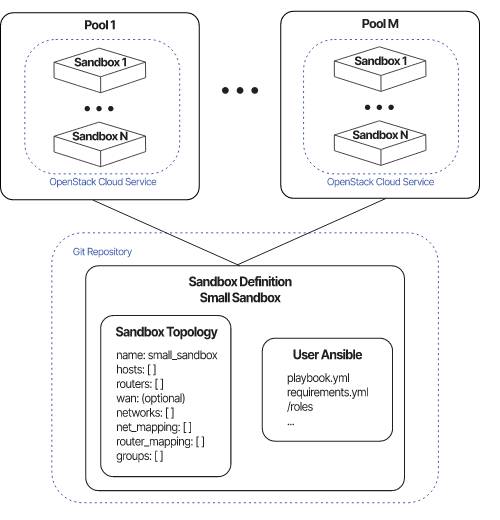
\includegraphics[width=0.92\linewidth,height=0.7\textheight,keepaspectratio]{src/images/KYPO-basic-elements-sandboxes.png}
  \caption{Kypo Basic Elements Sandboxes}
  \label{fig:KYPO-basic-elements-sandboxes}
\end{figure}


La creazione di una Sandbox si divide in 3 fasi:

\begin{itemize}
\tightlist
\item
  \textbf{Allocazione}: creazione della sandbox (=macchine virtuali)
  dentro al cloud.
\item
  \textbf{Networking}: setup della rete e distirbuzione delle chiavi di
  accesso dentro le macchine.
\item
  \textbf{Provisioning}: customizzazione delle macchine virtuali nella
  sandbox.
\end{itemize}

\begin{quote}
La creazione della Pool precede necessariamente la creazione delle
Sandbox.
\end{quote}

A partire dalla Topology Definition, viene prodotta la \textbf{Topology
Instance} utilizzando \passthrough{\lstinline!Terraform!} (che crea
l'infrastruttura virtuale). L'accesso alla topologia e' regolato da un
MAN (Management Access Node), ossia l'unico nodo connesso all'esterno
della rete della Topology Instance.

Di seguito, nell'immagine sburgoz, viene mostrata l'architettura
generale di una Topology Instance.

\begin{figure}[htbp]
  \centering
  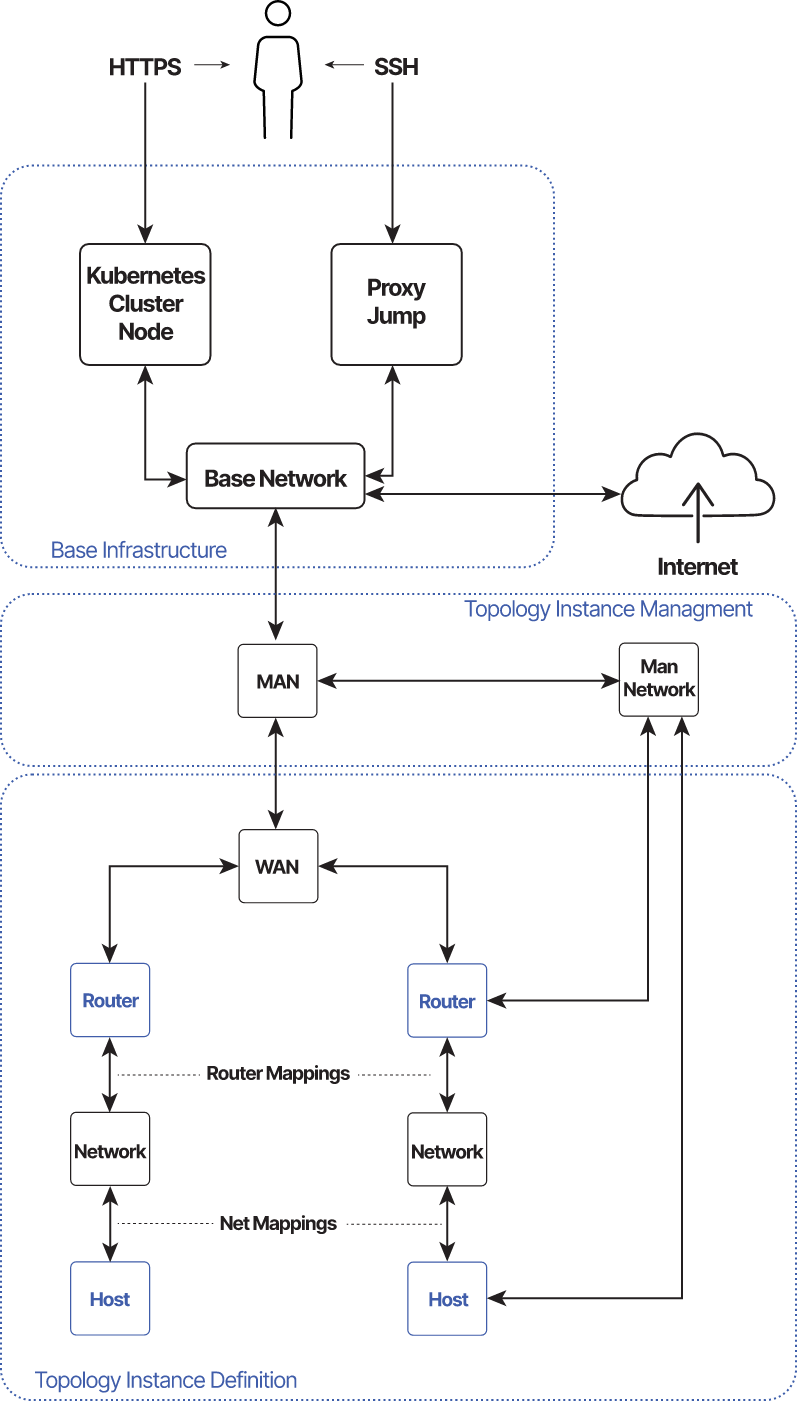
\includegraphics[width=0.92\linewidth,height=0.7\textheight,keepaspectratio]{src/images/KYPO-topology-instance.png}
  \caption{Kypo Topology Instance}
  \label{fig:KYPO-topology-instance}
\end{figure}


L'accesso alle macchine dentro la Sandbox e' regolato tramite SSH,
oppure da una console web accessibile via browser.

Gestire Sandobx, ossia intere Topology Instance e' costoso, infatti i
requisiti sono i seguenti:

\begin{itemize}
\tightlist
\item
  una macchina virtuale con almeno \emph{2 core CPU, 16 GB di RAM e 40
  GB di archiviazione}
\item
  un server dotato di almeno \emph{16 core CPU, 128 GB di RAM, 2 TB di
  archiviazione e almeno due interfacce di rete.}
\end{itemize}

Requisiti cosi alti sono necessari per:

\begin{itemize}
\tightlist
\item
  gestire l'infrastruttura OpenStack, i microservizzi, e Kubernetes
\item
  gestire l'esecuzione di centinaia di macchine virtuali e garantire la
  scalabilita al crescere degli utenti.
\end{itemize}

CyberRangeCZ a differenza di BlueAgent gestisce un'intera rete cloud, su
cui vengono orchestrati container, configurati dinamicamente con Ansible
e gestiti via Kubernetes, mentre BlueAgent e' un orchestratore di
container che esegue su un'unico host.

Di seguito sono illustrate le principali differenze tra CyberRangeCZ e
BlueAgent:

{\def\LTcaptype{none} % do not increment counter
\begin{longtable}[]{@{}
  >{\raggedright\arraybackslash}p{(\linewidth - 4\tabcolsep) * \real{0.3333}}
  >{\raggedright\arraybackslash}p{(\linewidth - 4\tabcolsep) * \real{0.3333}}
  >{\raggedright\arraybackslash}p{(\linewidth - 4\tabcolsep) * \real{0.3333}}@{}}
\toprule\noalign{}
\begin{minipage}[b]{\linewidth}\raggedright
Caratteristica
\end{minipage} & \begin{minipage}[b]{\linewidth}\raggedright
CyberRangeCZ
\end{minipage} & \begin{minipage}[b]{\linewidth}\raggedright
BlueAgent
\end{minipage} \\
\midrule\noalign{}
\endhead
\bottomrule\noalign{}
\endlastfoot
\textbf{Virtualizzazione} & Macchine Virtuali (VM) & Container di
sistema (Incus) \\
\textbf{Infrastruttura} & Cluster Cloud distribuito (OpenStack,
Kubernetes) & Singolo nodo host (Debian 13) \\
\textbf{Requisiti Hardware} & Elevati (16+ core, 128+ GB RAM, 2 TB
disco) & Minimi (eseguibile su singolo server o PC economico) \\
\textbf{Configurazione} & Runtime con Ansible e template Packer &
Creazione immagine con Distrobuilder \\
\textbf{Provisioning} & Lento (nell'ordine dei minuti) & Rapido
(nell'ordine dei secondi con CoW) \\
\textbf{Rete} & Rete virtuale OpenStack con nodo MAN & Linux Bridge L2,
WireGuard VPN e SDN OVN \\
\textbf{Verifica Difesa} & Non prevista nativamente & Cloni ZFS CoW su
switch OVN isolato \\
\textbf{Scopo Principale} & Emulazione reti aziendali e training su
larga scala & Cyber Range compatto per CTF di difesa \\
\end{longtable}
}
